\documentclass[FIPLY_base.tex]{subfiles}

\author{Gerald Irsiegler}
\date{26. Februar 2016}

\begin{document}
\section{Benutzerverwaltung}
\subsection{Beschreibung}
Die Applikation wurde als Single-User-Application entworfen und umgesetzt. In der Benutzerverwaltung kann der Benutzer seine
Daten angeben und umändern. Weiters kann er sein Social Media Profil mit der Applikation verbinden, um später Fortschritte mit seinen Freunden zu teilen.
Auch Daten welche essentiel zur Trainingsplanerstellung sind, werden hier aufgenommen.
\\\
\\\

\subsection{Aufteilung der Verwaltung}
Die Verwaltung bzw. Erstellung des Benutzers ist auf folgende drei Schritte aufgeteilt:

\subsubsection{Schritt 1}
Im ersten Schritt gibt der Benutzer seinen Namen und sein Geschlecht an.
Der Name wird in Plain Text eingegeben, während für das Geschlecht ein Spinner zur Verfügung gestellt wird, wobei man aus einer Liste aus: Male, Female und Other auswählen kann.
Weiters kann er sich hier über den Facebook-Login-Button mit seinem Facebook Account anmelden.
\\\
\\\
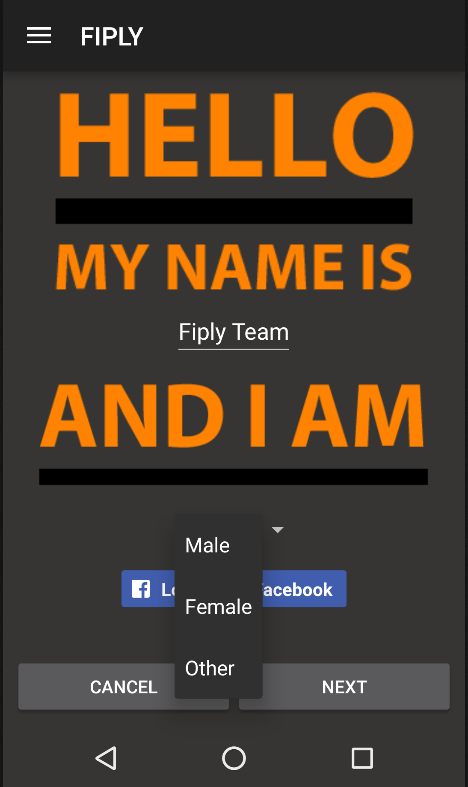
\includegraphics[scale=0.4]{img/User_step1}
\newpage
\subsubsection{Schritt 2}
Im zweiten Schritt gibt der Benutzer seine Körpergröße in Zentimetern (cm) und sein Gewicht in Kilogramm (kg) an.
\\\
\\\
Die Größe kann zwischen 100cm und 200cm auf jeden ganzen Wert eingestellt werden.
\\\
\\\
Das Gewicht kann zwischen 40kg und 140kg auf jeden ganzen Wert eingestellt werden.
\\\
\\\
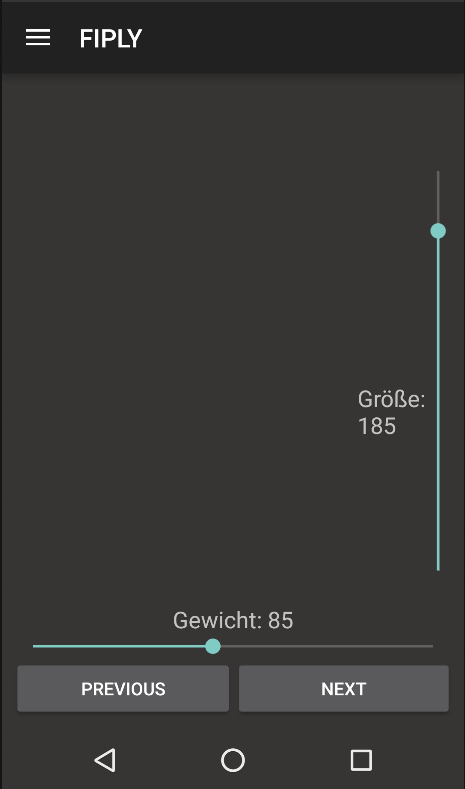
\includegraphics[scale=0.4]{img/User_step2}
\newpage
\subsubsection{Schritt 3}
Im dritten Schritt gibt der Benutzer an in welcher Altersgruppe er sich befindet und wie seine körperliche Verfassung derzeit ist.
Zur Auswahl stehen bei den Altersgruppen (in Jahren):
\begin{itemize}
\item 16-20
\item 21-30
\item 31-40
\item 41-50
\item 50+
\end{itemize}
Bei der derzeitigen Verfassung wird angegeben ob man körperlich fit oder unfit ist.
\\\
\\\
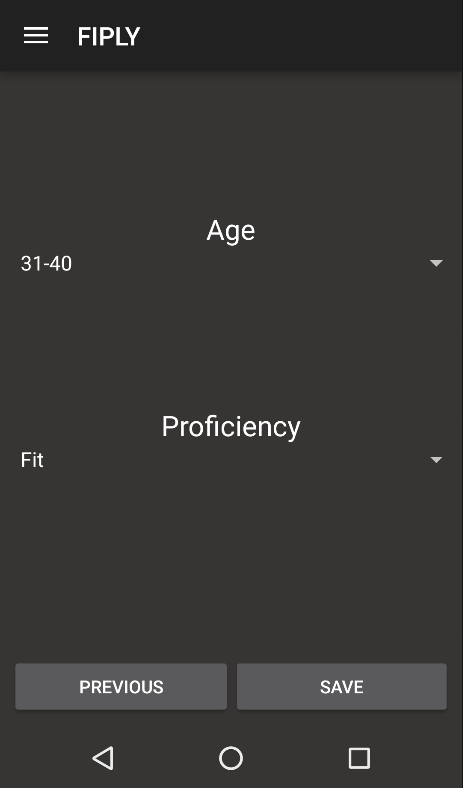
\includegraphics[scale=0.4]{img/User_step3}

\newpage

\subsection{Implementierung}
Alle Daten über den User werden im Key-Value-Repository der Datenbank als Key-Value-Paare abgespeichert. 
Weiters werden dei derzeit gespeicherten Werte automatisch eingetragen falls der Benutzer eine Seite erneut aufruft.

\end{document}
